\section{PSPACE}
\label{3DPSPACE}
In this section we show the PSPACE-completeness of 3D push-pull puzzles with equal push and pull strength. We will prove hardness by a reduction from True Quantified Boolean Formula (also known as TQBF and 3QSAT), which asks whether, given a set of variables $\{x_1, x_2, \ldots x_n, y_1, y_2, \ldots y_n\}$ and a boolean formula $\theta(x_1, \ldots x_n, y_1 \ldots y_n)$ in conjunctive normal form with exactly three variables per clause, the quantified boolean formula $\forall y_1 \exists x_1 \forall y_2 \exists x_2 \ldots \theta(x_1, \ldots x_n, y_1, \ldots y_n)$ is true.

We introduce a gadget called the 4-toggle and use it to simulate 3QSAT\cite{NPBook}. We construct the 4-toggle gadget in 3D push-pull block puzzles, completing the reduction. In particular we prove 3D Push1-Pull1 with thin walls is PSPACE-complete and 3D Push$i$-Pull$j$, for all positive $i=j$, is PSPACE-complete. A gap between NP and PSPACE still remains for 3D puzzles with different pull and push values, as well as for 2D puzzles. 

\subsection{Toggles}
We define an $n$-toggle to be a gadget which has $n$ internal pathways and can be in one of two internal states, $A$ or $B$. Each pathway has a side labeled $A$ and another labeled $B$. When the toggle is in the $A$ state, the pathways can only be traversed from $A$ to $B$ and similarly in the $B$ state it can only be traversed from $B$ to $A$. Whenever a pathway is traversed, the state of the toggle flips.


\begin{figure}[!ht]
\centering
\begin{subfigure}[t]{0.45\textwidth}
  \centering
    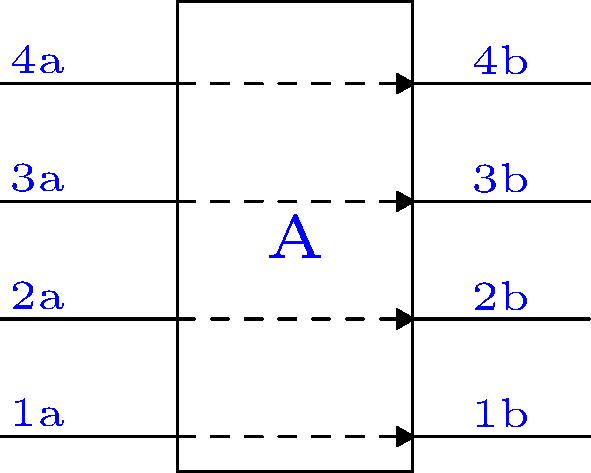
\includegraphics[width=0.8\textwidth]{Abstract4ToggleA}
    \caption{4-Toggle in state $A$. }%Here we can only follow the paths from left to right.
    \label{fig:Abstract4ToggleA}
\end{subfigure}
\begin{subfigure}[t]{0.45\textwidth}
  \centering
    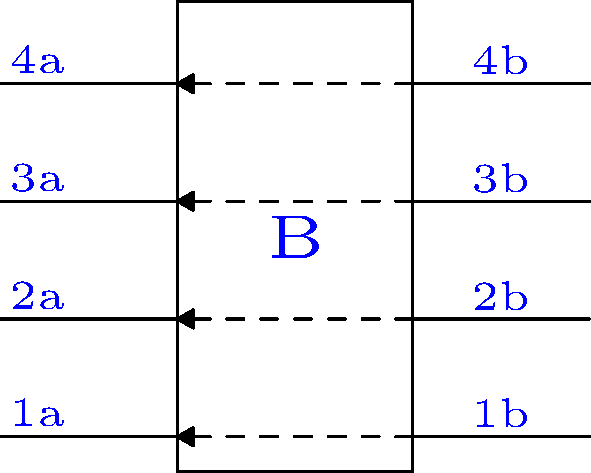
\includegraphics[width=0.8\textwidth]{Abstract4ToggleB}
    \caption{4-Toggle in state $B$. } %The direction of the paths through the toggle are flipped.
    \label{fig:Abstract4ToggleB}
\end{subfigure}
\caption{Diagrams of the two possible states of a 4-Toggle.}
\label{fig:4-toggle}
\end{figure}

\begin{figure}[!ht]
\centering
\begin{subfigure}[t]{0.45\textwidth}
  \centering
    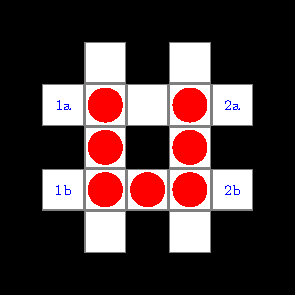
\includegraphics[width=0.8\textwidth]{2Toggle}
    \caption{2-Toggle in state $A$. The arrows indicate the transition to state $B$.}
    \label{fig:2toggleA}
\end{subfigure}
\begin{subfigure}[t]{0.45\textwidth}
  \centering
    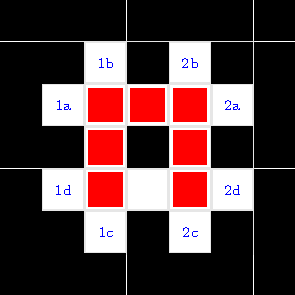
\includegraphics[width=0.8\textwidth]{2ToggleB}
    \caption{2-Toggle in state $B$.}
    \label{fig:2toggleB}
\end{subfigure}

    \caption{2-Toggles constructed in a push-pull block puzzle.}
\end{figure}


\begin{table}
\begin{minipage}{.45\textwidth}
\centering
{\setlength\tabcolsep{4pt}
\begin{tabular}{>{$} l <{$} >{$} l <{$} >{$} l <{$} >{$} l <{$}}
   A: & & & \\
   &(A, 1a)& \rightarrow& (B, 1b) \\
   &(A, 2a)& \rightarrow & (B, 2b) \\
   &(A, 3a)& \rightarrow& (B, 3b) \\
   &(A, 4a)& \rightarrow & (B, 4b)  \\ \\
\end{tabular}}
\end{minipage}
\begin{minipage}{.45\textwidth}
\centering
{\setlength\tabcolsep{4pt}
\begin{tabular}{>{$} l <{$} >{$} l <{$} >{$} l <{$} l}
   B: & & & \\
   &(B, 1b)& \rightarrow& (A, 1a) \\
   &(B, 2b)& \rightarrow & (A, 2a) \\
   &(B, 3b)& \rightarrow& (A, 3a) \\
   &(B, 4b)& \rightarrow & (A, 4a)  \\ \\
\end{tabular}}
\end{minipage}
\caption{State transitions of a 4-toggle as seen in Figure~\ref{fig:4-toggle}}
\label{4ToggleStateTransition}
\end{table}

Figure~\ref{fig:2toggleA} acts as a 2-toggle. The locations $1a$, $1d$, $2a$, and $2d$, are all entrances and exits to the 2-toggle, while $1b$ connects directly to $1c$, and $2b$ connects directly to $2c$. Notice that there is a single block missing from the ring of eight blocks. When the missing block is on top, as diagrammed, it will represent state $A$, and when it is on the opposite side, we call it state $B$. Notice that in state $A$, it is impossible to enter through entries $1d$ or $2d$. When we enter in the $1a$ or $2a$ sides, we can follow the moves in the series of diagrams to exit the corresponding $1d$ or $2d$ side, leaving the gadget in the $B$ state. One can easily check that the gadget can only be left in either state $A$, $B$, or a broken state with the empty square left in a corner. Notice that in the broken state, every pathway except the one just exited is blocked. If we enter through that path, it is in exactly the same state as if it had been in an allowed state and entered through the corresponding pathway normally. For example, in the diagram one can only enter through $1a$ and after doing so the blocks are in the same position as they would be after entering in path $1a$ on a 2-toggle in state $A$. Thus the broken state is never more useful for solving the puzzle and can be safely ignored. To generalize to Push-$k$ Pull-$k$ we simply expand the number of blocks between entrances and exists. Instead of having $3$ blocks between each entrance and exit, we have $2k+1$ blocks. There is still one vacant square left in the center of one of the rows of blocks to dictate the state of the toggle. The robot can push the row of $k$ blocks to the center or pull $k$ blocks opening up a square in the center, giving us the same function as before.

To construct a 4-toggle we essentially take two copies of the 2-toggle, rotate them perpendicular to each other in 3D, and let them overlap on the central axis, where the block is missing. See Figure~\ref{fig:4Toggle3D}. We still interpret the lack of blocks in the same positions as in the 2-toggle as states $A$ or $B$. 
For Push1-Pull1, this construction requires thin walls, since the exit pathways from $1b$, $2b$, $3b$ and $4b$ must pass immediately next to each other. For Push$k$-Pull$k$, with $k > 1$, thin walls are not necessary, since the exit pathways are separated from each other.
\subsection{Locks}

A 2-toggle and lock is a gadget consisting of a 2-toggle and a separate pathway. Traversing the separate pathway is only possible if the 2-toggle is in a specific state, and the traversal does not change the internal state of the 2-toggle. The 2-toggle functions exactly as described above.

This gadget can be implemented using a 4-toggle by
connecting the $3b$ and $4b$ entrances of the 4-toggle with an additional corridor, as shown in Figure~\ref{fig:LockA}.
Traversing the resultant full pathway, from $3a$ to $3b$ to $4b$ to $4a$, is possible only if the initial
state of the 4-toggle is $A$, and will leave the 4-toggle in state $A$. In addition, a partial traversal,
such as from $3a$ to $3b$ and back to $3a$, does not change the internal state. The two unaffected
pathways of the toggle, $1$ and $2$, continue to function as a 2-toggle.

A 2-toggle and lock can be extended to a 2-toggle with many locks. The 2-toggle with many locks is a gadget consisting of a 2-toggle and any number of separate pathways which can only be traversed when the gadget is in state $B$. This can be constructed using one 2-toggle and lock per separate pathway needed and attaching the toggles in series.
We orient the 2-toggles so that their 2-toggles are all passable at once in one direction.
When the 2-toggle is traversed, all of the internal locks' states flip, rendering the gadget passable in the opposite direction, and switching the passability and impassibility of all of the external pathways.

\subsection{Quantifiers}


\subsubsection{Existential Quantifier}
An existential gadget is like a 2-toggle and many locks, except that instead of a
2-toggle, it has a single pathway which is always passable in both directions. Upon traversing the pathway
the robot may or may not change the internal state of the 2-toggle and many locks, as it chooses. The variable is 
considered true if the 2-toggles and many locks is in state $A$ and false if it is in state $B$. This gadget
is shown in Figure~\ref{fig:Existential}.

\subsubsection{Alternating Quantifier Chain}
\begin{figure}[h!]
\centering
    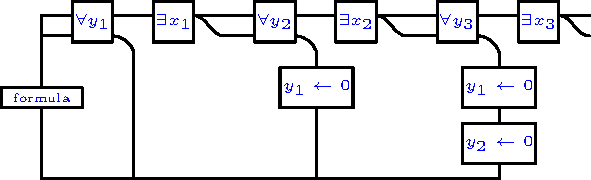
\includegraphics[width=0.9\textwidth]{QuantifierChain}
    \caption{A segment of the alternating quantifier chain. Each square represents the 2-toggle part of a 2-toggle and many locks.}
    \label{fig:QuantifierChain}
\end{figure}

An alternating quantifier chain, shown in Figure~\ref{fig:QuantifierChain}, implements a series of
alternating existential and universal variables, as well as external literal pathways, which may be traversed
if and only if their corresponding variables are set to a prespecified value.

Traversing the quantifier chain
repeatedly in the primary direction will cycle the universal variables through all $2^n$ possible settings.
Upon each traversal, an initial sequence of the universal variables will have their values flipped.
During the traversal, the robot will have the option to set a series of corresponding existential variables to whatever value it wishes. These comprise the existentials nested within the universal variables whose values were flipped. An analysis of the Quantifier Chain can be found in Appendix~\ref{sec:AnalysisQuantifierChain}

\subsection{Clause Gadget}
We construct a clause gadget by putting lock pathways of three 2-toggle with many locks in parallel, as we did with Set-Verify gadgets in Figure~\ref{fig:NPClauseGadget}. Each of these paths can be traversed only if the corresponding variable has been set to true, or to false, depending on the orientation of that particular lock. Since they are in parallel, only one needs to be passable for the robot to be able to continue on to the next clause.

\subsection{Beginning and End Conditions}
The overall progression of the robot through the puzzle starts with the quantifier chain.
The robot increments the universal variables and sets the appropriate existential variables arbitrarily, 
then traverses a series of clause gadgets to verify that the TQBF formula represented by those clauses 
is true under that setting of the variables. Then, the robot cycles around to the quantifier chain, and repeats.

At the beginning of this procedure, the robot must be allowed to set all of the existential variables arbitrarily.
To ensure this, we will set up the quantifier gadget in the state $01 \ldots 11$, with all variables set to $1$
except the highest order one.  The highest order variable will be special, and will not be used in the $3CNF$
formula. The initial position of the robot will be at the entrance to the quantifier gadget. This will allow
the robot to flip every universal in the quantifier gadget, from $01 \ldots 11$ to $10 \ldots 00$, and accordingly
set every existential variable arbitrarily. To force the robot to go forward through the quantifier gadget
instead of going backwards through the clause chain, we will add a literal onto the end of the formula gadget
which is passable if and only if the highest order variable is set to $1$.
After this set up, the robot will progress through the loop consisting of the quantifier gadget and the
formula gadget, demonstrating the appropriate existential settings for each assignment of the universal
quantifiers.

At each point in this process, the robot has the option to proceed through this cycle backwards, as is
guaranteed by the reversibility of the game. However, at no point does proceeding in the reverse direction
give the robot the ability to access locations or set toggles to states that it could not have performed
when it initially encountered the toggles or locations. Thus, any progression through the states of the
alternating quantifier chain must demonstrate a TQBF solution to the formula given.

After progressing through every possible state of the universal quantifiers, the universals will be in the
state $11 \ldots 11$. At this point, the robot may progress through the quantifier gadget and exit via its special
pathway,
the carry pathway of the highest order bit. This special pathway will lead to the goal location of the puzzle.
Thus, only by traversing the quantifier - formula loop repeatedly, and demonstrating the solution to the TQBF
problem,
will the robot be able to reach the goal. The robot may reach the goal if and only if the corresponding quantified
boolean formula is true.

\begin{theorem}
    \label{thm:3dPSPACE-complete}
    Push-$k$ Pull-$k$, $k>1$ in 3D with fixed blocks is PSPACE-complete.
\end{theorem}
\begin{proof}
By the above construction, TQBF can be reduced to Push-$k$ Pull-$k$ in three dimensions with fixed walls, through the intermediate step of construction a 4-toggle. This implies that Push$k$-Pull$k$ is PSPACE-hard.
Since Push$k$-Pull$k$ has a polynomial-size state, the problem is in NPSPACE, and therefore in PSPACE by Savitch's Theorem\cite{SAVITCH1970177}. So it is PSPACE-complete.
\end{proof}

\begin{theorem}
    Push-1 Pull-1 in 3D with thin walls is PSPACE-complete.
\end{theorem}
\begin{proof}
    Push-1 Pull-1 in 3D with thin walls can construct a 4-toggle, and so by the same argument as in Theorem~\ref{thm:3dPSPACE-complete}, it is PSPACE-complete.
\end{proof}
